\chapter{Desenvolvimento}\label{chp:desenvolvimento}

Para realização da solução proposta nesse trabalho, é necessário o desenvolvimento de um aplicativo móvel para que o rastreamento de doenças infecciosas ocorra de forma automática. Assim, na seção X ...

\section{Levantamento e Análise de Requisitos}\label{sec:requisitos}
% Levantamento e Análise de Requisitos (lista de requisitos func e não func + casos de uso)

O aplicativo deve automatizar todo o ciclo do rastreamento, desde a captura da exposição à uma doença, até a notificação feita à pessoa possivelmente exposta. Com isso, a partir do problema de rastreamento de contatos apresentado no Capítulo \ref{chp:Introducao}, o processo de análise de requisitos foi feito pensando nos possíveis casos de uso do usuário.

Como o aplicativo utiliza um sistema de \textit{check-in}, os usuários necessitam de um buscador para encontrar os locais que foram visitados. Esse buscador deve estar relacionado a uma extensa \Sigla{Base de Dados}{BD} para que a maioria dos locais inseridos pelos usuários sejam encontrados. Por conta disso, uma BD externa deve ser utilizada, já que a criação de uma nova não traria a experiência esperada para o usuário.

Depois que a busca foi feita, o usuário deve ser capaz de salvar o local encontrado. O salvamento deve ser feito em uma BD remota, para que a rotina de checagem do rastreamento de contatos seja feita no servidor. Com isso, o dispositivo móvel do usuário não precisará de conectividade com a \textit{internet}, nem que o aplicativo rode em segundo plano durante a execução da rotina, evitando o consumo desnecessário de bateria do dispositivo.

Se um usuário for infectado por uma doença, ele deve ser capaz de declarar no aplicativo que está infectado. A partir disso, a rotina de rastreamento de contatos deve ser capaz de relacionar os locais do usuário infectado com os usuários comuns, procurando por algum possível contato que possa ter ocorrido.

O usuário deve receber notificações caso o mesmo tenha tido algum possível contato com outras pessoas que utilizam o aplicativo e estavam infectadas. Essa notificação deve ser enviada de forma automática e sem a necessidade de intervenção humana, para que o problema seja resolvido de forma automática de ponta a ponta.

A partir de toda análise acima, foram levantados 4 requisitos funcionais, que são:

\begin{enumerate}
  \item Buscar localizações;
  \item Salvar localizações;
  \item Declarar caso de infecção confirmado;
  \item Enviar notificação de exposição;
  %\item Autenticar usuário
\end{enumerate}

Esses requisitos englobam todo o ciclo do rastreamento e estão representados na \Figura{fig:casosdeuso}.

%\caption[Legenda curta de figura]{Legenda longa da figura.}
\begin{figure}[!htb]
\centering
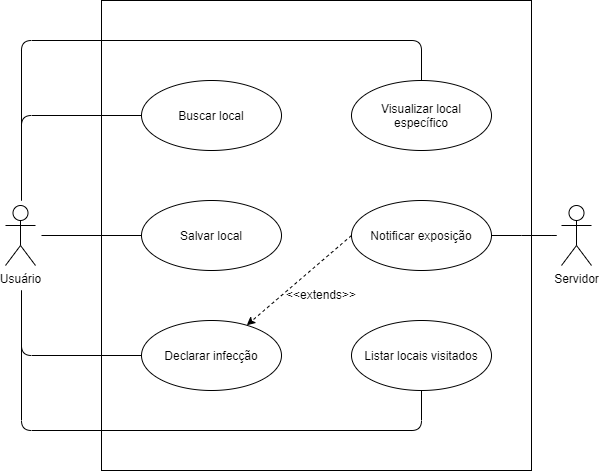
\includegraphics[scale=0.7]{Diagrama de casos de uso.png}
\caption{Diagrama de casos de uso da aplicação.}
\label{fig:casosdeuso}
\end{figure}

Além dos requisitos funcionais, existem outros pontos a serem analisados na solução proposta do problema explicitado no Capítulo \ref{chp:Introducao}.

O primeiro ponto é que a eficácia da solução depende diretamente do número de usuários que utilizarem o aplicativo. Por conta disso, o aplicativo deve funcionar em diferentes tipos de sistema operacionais de dispositivos móveis, a fim de atingir a maior quantidade de usuários.

Para que esse requisito seja atendido, o aplicativo pode ser desenvolvido especialmente para cada tipo de \Sigla{Sistema Operacional}{SO} ou utilizando um \textit{framework} híbrido, em que a partir da mesma base de código é possível construir os arquivos para cada SO.

Além disso, como o aplicativo armazena todas as localizações recentemente frequentadas pelos usuários que efetuarem os \textit{check-ins}, ele deve se preocupar em garantir a segurança desses dados.

A segurança dos dados armazenados pela aplicação será garantida a partir da utilização de criptografia. Ela será aplicada aos dados em trânsito e em repouso, ou seja, tanto durante a comunicação entre cliente e servidor quanto no armazenamento na BD.

Ainda relacionado à segurança, a fim de preservar a privacidade das pessoas que utilizarem o aplicativo, a aplicação ou os usuários não devem ser capazes de descobrir quem possivelmente expôs outras pessoas a alguma doença. Isso significa que quando um usuário receber uma notificação de exposição, ele não será capaz de identificar quem foi, nem o local que isso ocorreu.

Para isso, o aplicativo não terá a inserção de nenhum dado pessoal, ou seja, a autenticação será feita de forma anônima, onde cada usuário será representado por uma cadeia de caracteres aleatórios.

Por último, toda localização terá prazo de validade de 14 dias. Isso significa que todo \textit{check-in} efetuado pelo usuário será armazenado apenas durante esse prazo. Como a solução do problema é a automação do rastreamento de contatos, localizações mais antigas do que esses dias não são necessárias, já que o período de transmissão do vírus haveria terminado.

A partir do que foi explicado nos parágrafos anteriores, foram levantados 3 requistos não funcionais. Esses requisitos são:
\begin{enumerate}
  \item Compatibilidade multiplataforma;
  \item Garantia de privacidade e segurança dos dados;
  \item Exclusão de localizações antigas;
\end{enumerate}

\section{Modelagem}\label{sec:modelagem}
% Modelagem (arquitetura, diagrama de classes, modelagem de dados)

\section{Implementação}\label{sec:implementacao}
